\section{Results and Discussion}
\label{sec:results}

\subsection{Benchmark Performance Comparison}
We evaluate our proposed SHAP-DA-IDS framework against five comparative configurations on the 71,591 holdout test connections of the DS2OS dataset. Table~\ref{tab:model_comparison} reports the overall performance metrics, and Fig.~\ref{fig:model_comparison} compares the macro F1-score and raw accuracy across models.

\begin{table}[!t]
\centering
\caption{Benchmark Model Performance on DS2OS Test Set (71,591 Samples)}
\label{tab:model_comparison}
\begin{tabular}{|l|c|c|c|c|}
\hline
\textbf{Model Configuration} & \textbf{Acc. (\%)} & \textbf{Macro F1 (\%)} & \textbf{W-F1 (\%)} & \textbf{AUC} \\ \hline
Logistic Regression & 97.73 & 29.97 & 96.89 & 0.8415 \\ \hline
Random Forest & \textbf{97.84} & \textbf{31.08} & \textbf{97.10} & 0.8675 \\ \hline
XGBoost (Unbalanced) & 97.79 & 22.71 & 97.06 & \textbf{0.8905} \\ \hline
XGBoost + Class Weights & 47.48 & 15.28 & 62.74 & 0.8509 \\ \hline
XGBoost + Fixed (DIFT) & 97.81 & 29.04 & 97.07 & 0.8891 \\ \hline
\textbf{SHAP-DA-IDS (Ours)} & 97.76 & 29.17 & 97.09 & 0.8770 \\ \hline
\end{tabular}
\end{table}

\begin{figure}[!t]
\centering
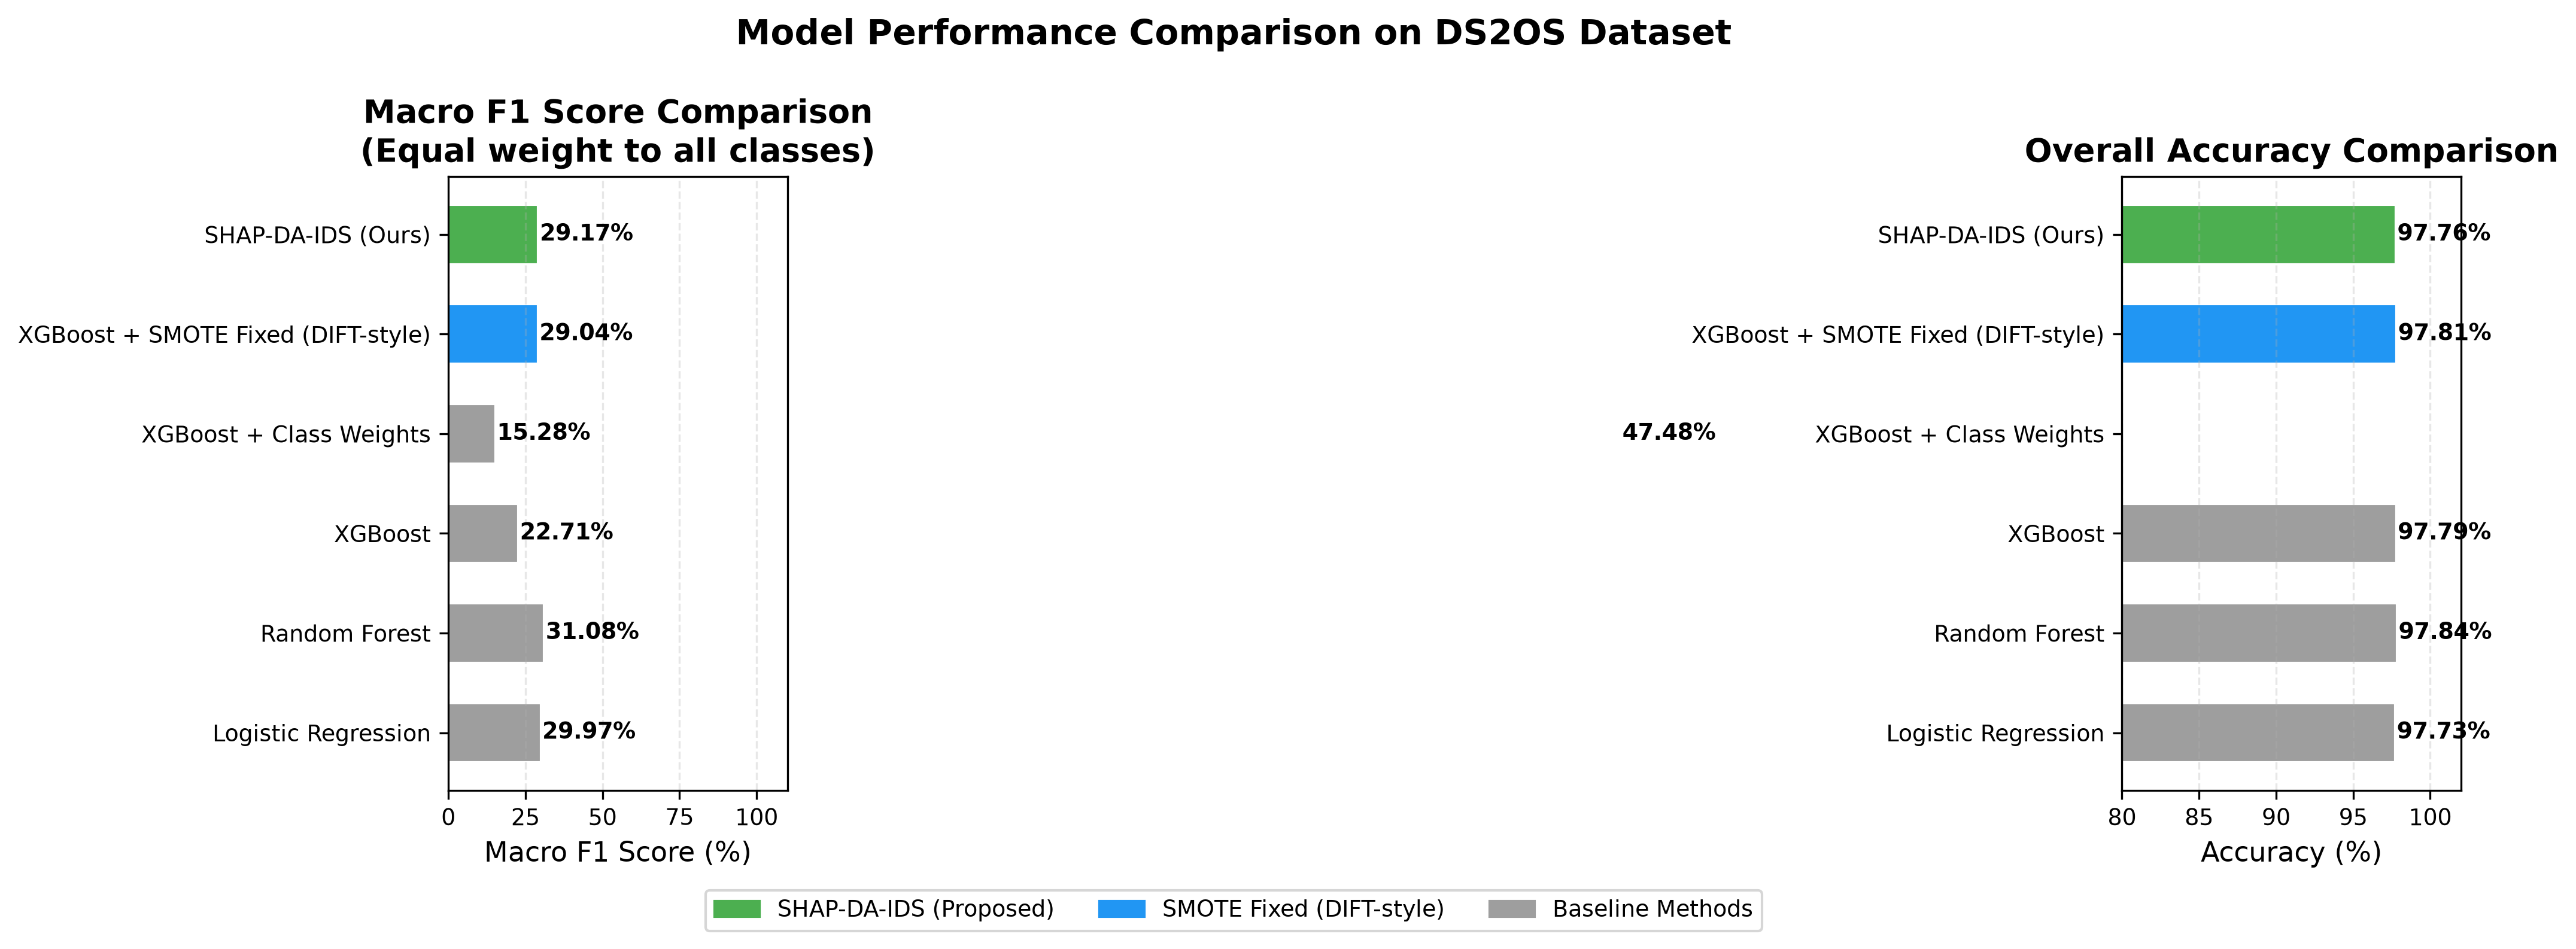
\includegraphics[width=\columnwidth]{images/3.png}
\caption{Macro F1-score (left) and overall classification accuracy (right) across all evaluated baseline and proposed models on the DS2OS test split.}
\label{fig:model_comparison}
\end{figure}

Several clear trends emerge from these benchmark comparisons:
\begin{enumerate}
    \item \textbf{Overall Accuracy is Misleading:} Nearly all models achieve overall accuracy between 97.73\% and 97.84\%. However, because normal traffic accounts for 97.20\% of all records, a naive classifier that simply labels every flow as normal achieves 97.20\% accuracy while failing to catch even a single attack. Macro F1-score provides a much more honest measure of real-world utility by weighting all eight classes equally regardless of their size.
    \item \textbf{Failure of Simple Cost Weighting:} Training XGBoost with inverse class frequency weights causes overall accuracy to plummet from 97.79\% to 47.48\%, with weighted F1 dropping to 62.74\%. While this aggressive reweighting forces the model to predict minority classes more often, it generates an overwhelming number of false alarms on normal traffic (normal recall falls to 47.35\%). In an operational environment, an alert flood of this scale would overwhelm security operators.
    \item \textbf{Clear Gain over Raw Boosting:} Our proposed SHAP-DA-IDS lifts the macro F1-score from 22.71\% on raw unbalanced data to 29.17\% (+6.46\% absolute gain), confirming that intelligent data augmentation is necessary when classes are this severely skewed.
\end{enumerate}

\subsection{Minority Attack Detection}
The primary objective of this work is to help intrusion detection systems spot rare, subtle attacks that standard training misses. Table~\ref{tab:per_class} details the per-class F1-scores across all eight categories, and Fig.~\ref{fig:per_class} focuses specifically on the seven minority attack types.

\begin{table}[!t]
\centering
\caption{Per-Class F1-Score (\%) Breakdown on Test Set (71,591 Samples)}
\label{tab:per_class}
\begin{tabular}{|l|c|c|c|c|}
\hline
\textbf{Class Label} & \textbf{Test Count} & \textbf{Unbalanced} & \textbf{DIFT Fixed} & \textbf{Ours} \\ \hline
Data Probing & 68 & 0.00 & 0.00 & \textbf{4.60} \\ \hline
DoS & 1,156 & 55.25 & 55.29 & \textbf{55.93} \\ \hline
Malicious Control & 178 & 3.26 & 2.14 & \textbf{9.61} \\ \hline
Malicious Operation & 161 & 0.00 & 0.00 & 0.00 \\ \hline
Normal & 69,588 & 98.91 & \textbf{98.92} & 98.90 \\ \hline
Scan & 310 & 0.00 & 0.00 & 0.00 \\ \hline
Spying & 106 & 0.00 & 0.00 & 0.00 \\ \hline
Wrong Setup & 24 & 24.24 & \textbf{76.00} & 64.29 \\ \hline
\end{tabular}
\end{table}

\begin{figure}[!t]
\centering
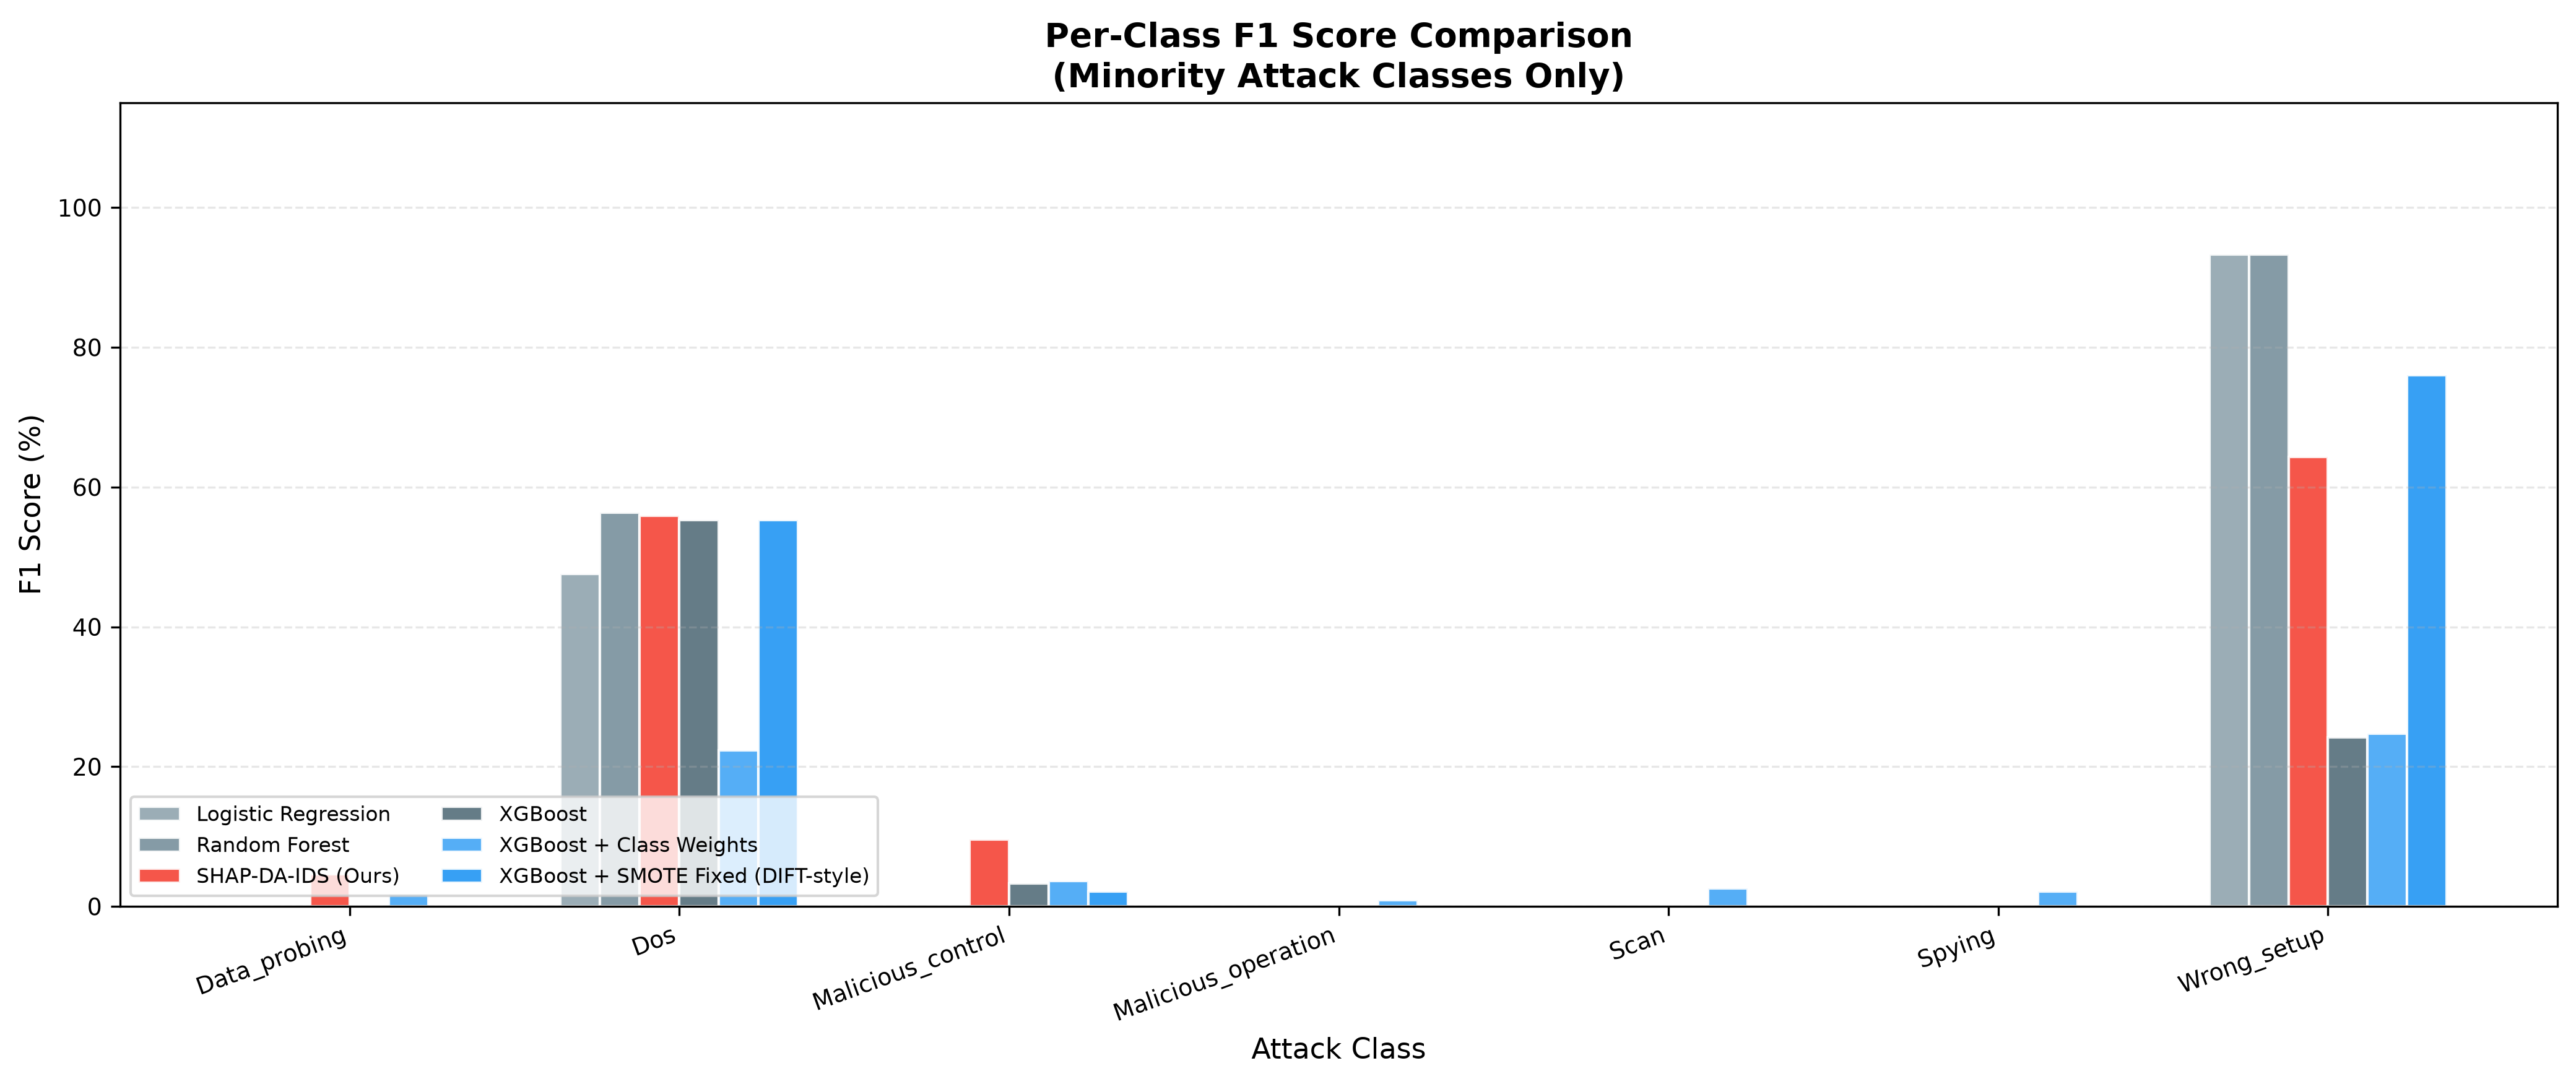
\includegraphics[width=\columnwidth]{images/5.png}
\caption{Per-class F1-score comparison across the seven minority attack categories, highlighting the gains achieved on rare attack vectors.}
\label{fig:per_class}
\end{figure}

The per-class breakdown reveals two key improvements:
\begin{itemize}
    \item \textbf{Breakthrough on Data Probing:} Logistic Regression, Random Forest, Unbalanced XGBoost, and DIFT-style fixed augmentation all achieve an F1-score of exactly 0.00\% on Data Probing (68 test samples). Because Data Probing represents only 0.096\% of the training data, these models simply never predict it. In contrast, SHAP-DA-IDS achieves an F1-score of 4.60\% with 10.53\% precision, establishing the first viable detection boundary for this attack.
    \item \textbf{4.49$\times$ Improvement on Malicious Control:} Malicious Control represents unauthorized actuation commands sent to smart devices (e.g., unlocking a door or altering an actuator setting). Under DIFT-style fixed augmentation, the F1-score is only 2.14\%. Under our difficulty-adaptive augmentation, the F1-score reaches \textbf{9.61\%} (21.57\% precision, 6.18\% recall), representing more than a fourfold improvement.
    \item \textbf{Normal Traffic Specificity Preserved:} Crucially, expanding the minority training samples did not degrade the model's ability to recognize normal traffic. Normal precision remains at 98.00\%, recall is 99.82\%, and the F1-score is 98.90\%.
\end{itemize}

Fig.~\ref{fig:confusion_matrix} presents the confusion matrix for SHAP-DA-IDS on the test partition, showing both raw prediction counts and normalized percentages.

\begin{figure}[!t]
\centering
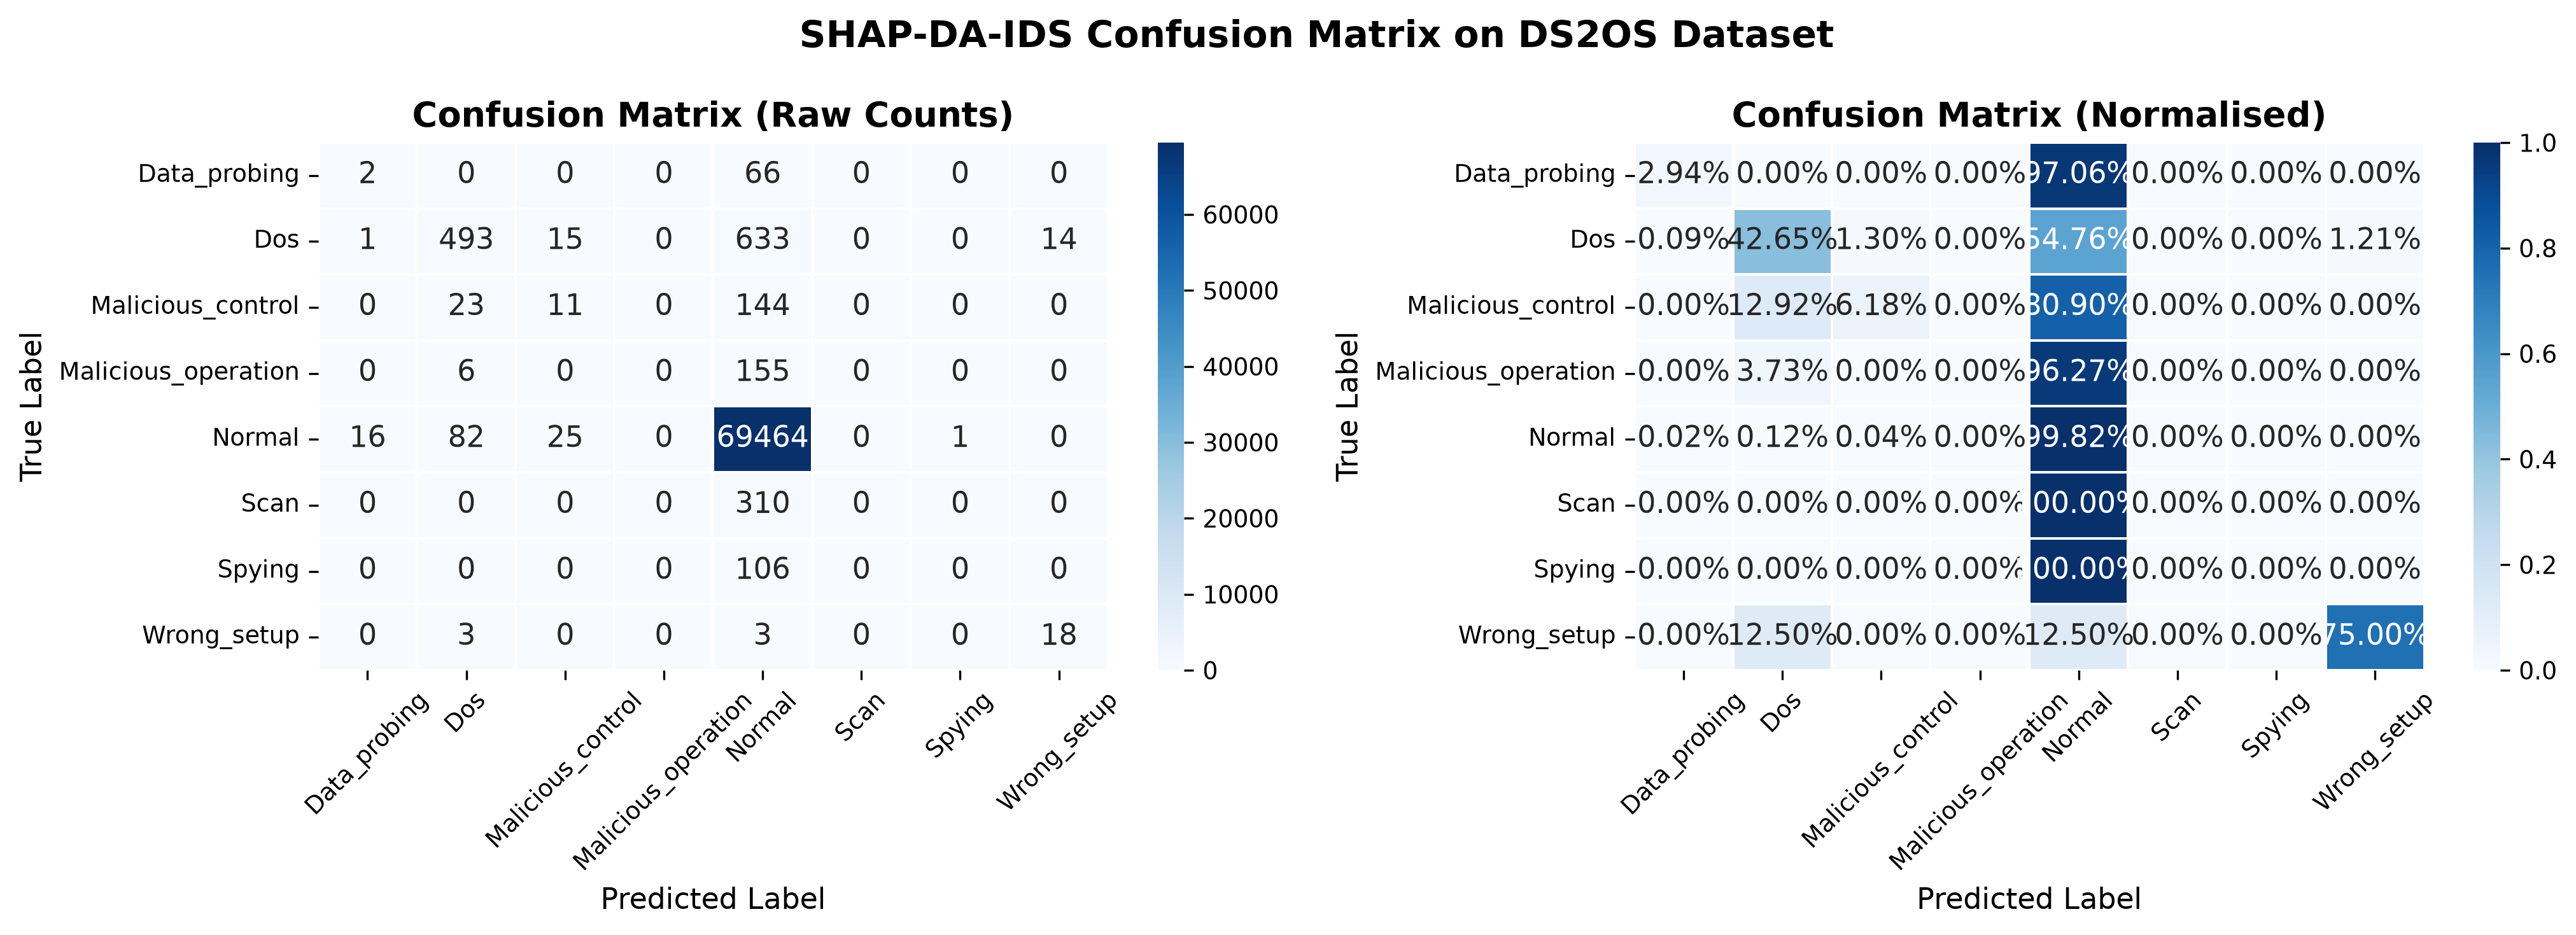
\includegraphics[width=\columnwidth]{images/4.png}
\caption{Confusion matrix of SHAP-DA-IDS on the test set: raw connection counts (left) and normalized classification percentages (right).}
\label{fig:confusion_matrix}
\end{figure}

\subsection{Why Adaptive Quotas Outperform Fixed Augmentation}
To understand why SHAP-DA-IDS outperforms DIFT's augmentation approach, Table~\ref{tab:strat_comparison} and Fig.~\ref{fig:aug_strat} compare their respective synthetic target allocations alongside the empirical difficulty ratings from cross-validation.

\begin{table}[!t]
\centering
\caption{Synthetic Target Allocations: Fixed (DIFT) vs. Adaptive (Ours)}
\label{tab:strat_comparison}
\begin{tabular}{|l|c|c|c|c|}
\hline
\textbf{Class Label} & \textbf{Raw Train} & \textbf{Prelim F1} & \textbf{DIFT} & \textbf{Adaptive} \\ \hline
Data Probing & 274 & 0.0215 & 1,144 & 14,552 \\ \hline
DoS & 4,624 & 0.2087 & 4,624 & 16,170 \\ \hline
Malicious Control & 711 & 0.0266 & 1,144 & 14,914 \\ \hline
Malicious Operation & 644 & 0.0086 & 1,144 & 15,110 \\ \hline
Normal & 278,347 & 0.8666 & 278,347 & 278,347 \\ \hline
Scan & 1,237 & 0.0349 & 1,237 & 15,319 \\ \hline
Spying & 426 & 0.0271 & 1,144 & 14,623 \\ \hline
Wrong Setup & 98 & 0.9500 & 1,144 & 827 \\ \hline
\end{tabular}
\end{table}

\begin{figure}[!t]
\centering
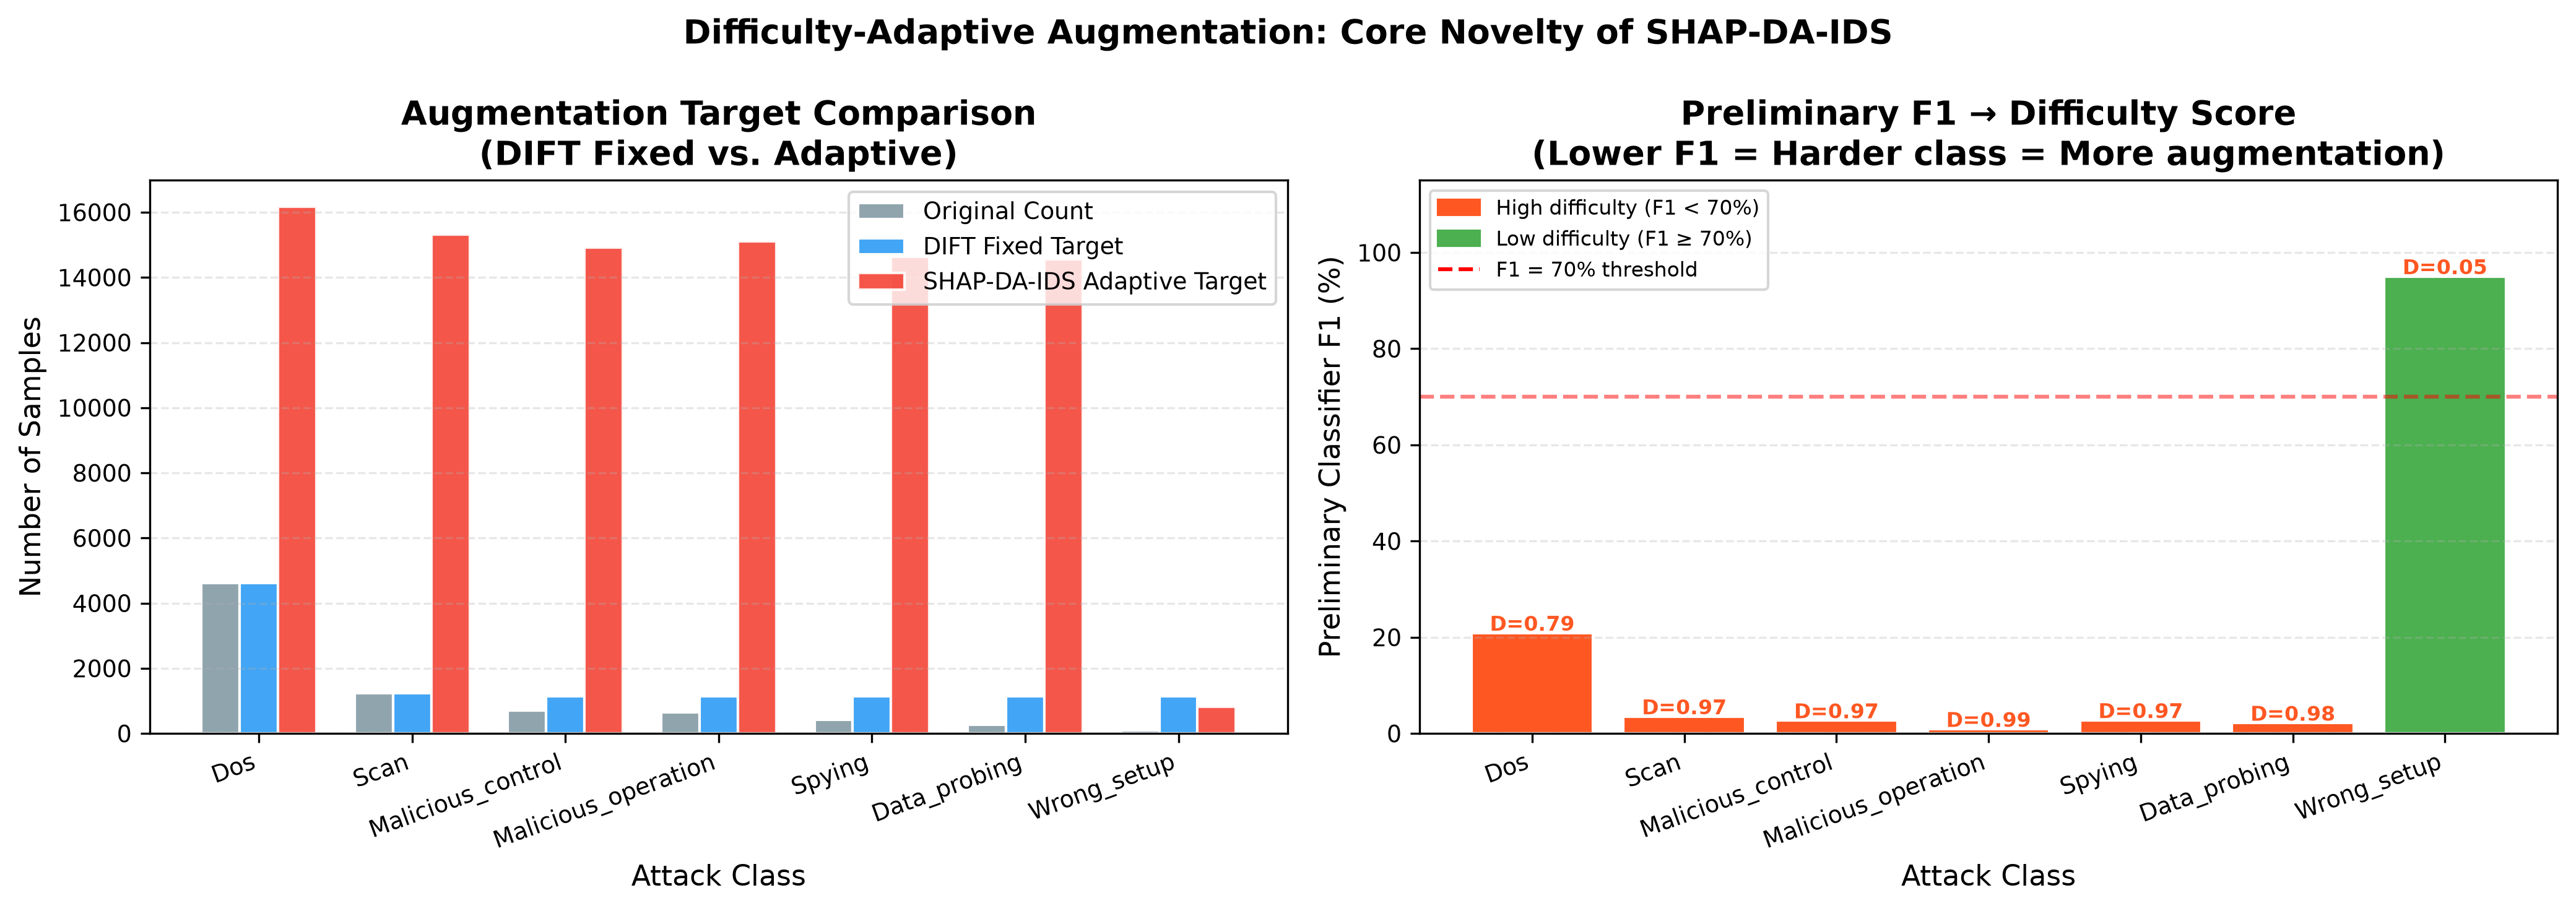
\includegraphics[width=\columnwidth]{images/7.png}
\caption{Difficulty-Adaptive Augmentation mechanism: target sample quotas (left) and preliminary cross-validation F1-scores defining class difficulty (right).}
\label{fig:aug_strat}
\end{figure}

Under DIFT's rule, the augmentation quota for every minority class is clamped to the arithmetic average of all minority counts (1,144 samples). Consequently, Data Probing is increased by only 870 samples, and Malicious Control by 433 samples. Against 278,347 normal samples, normal traffic still outnumbers them by more than 240 to 1, leaving the decision boundary completely overwhelmed.

In contrast, our difficulty-adaptive formula observes that Data Probing and Malicious Control have preliminary F1-scores near zero ($D_c > 0.97$) and allocates them approximately 14,500 to 15,000 samples. Meanwhile, Wrong Setup already achieves a preliminary F1-score of 0.95 ($D_c = 0.05$), so our formula assigns it only 827 samples. This prevents wasteful synthesis on classes that the model can already separate easily, directing the generation budget where it is needed most.

\subsection{Threat Attribution via TreeSHAP}
A key limitation of DIFT is that it operates as a black box. In contrast, SHAP-DA-IDS provides post-hoc feature explanations using TreeSHAP. Fig.~\ref{fig:shap_importance} illustrates the global feature importance rankings across all test-set predictions.

\begin{figure}[!t]
\centering
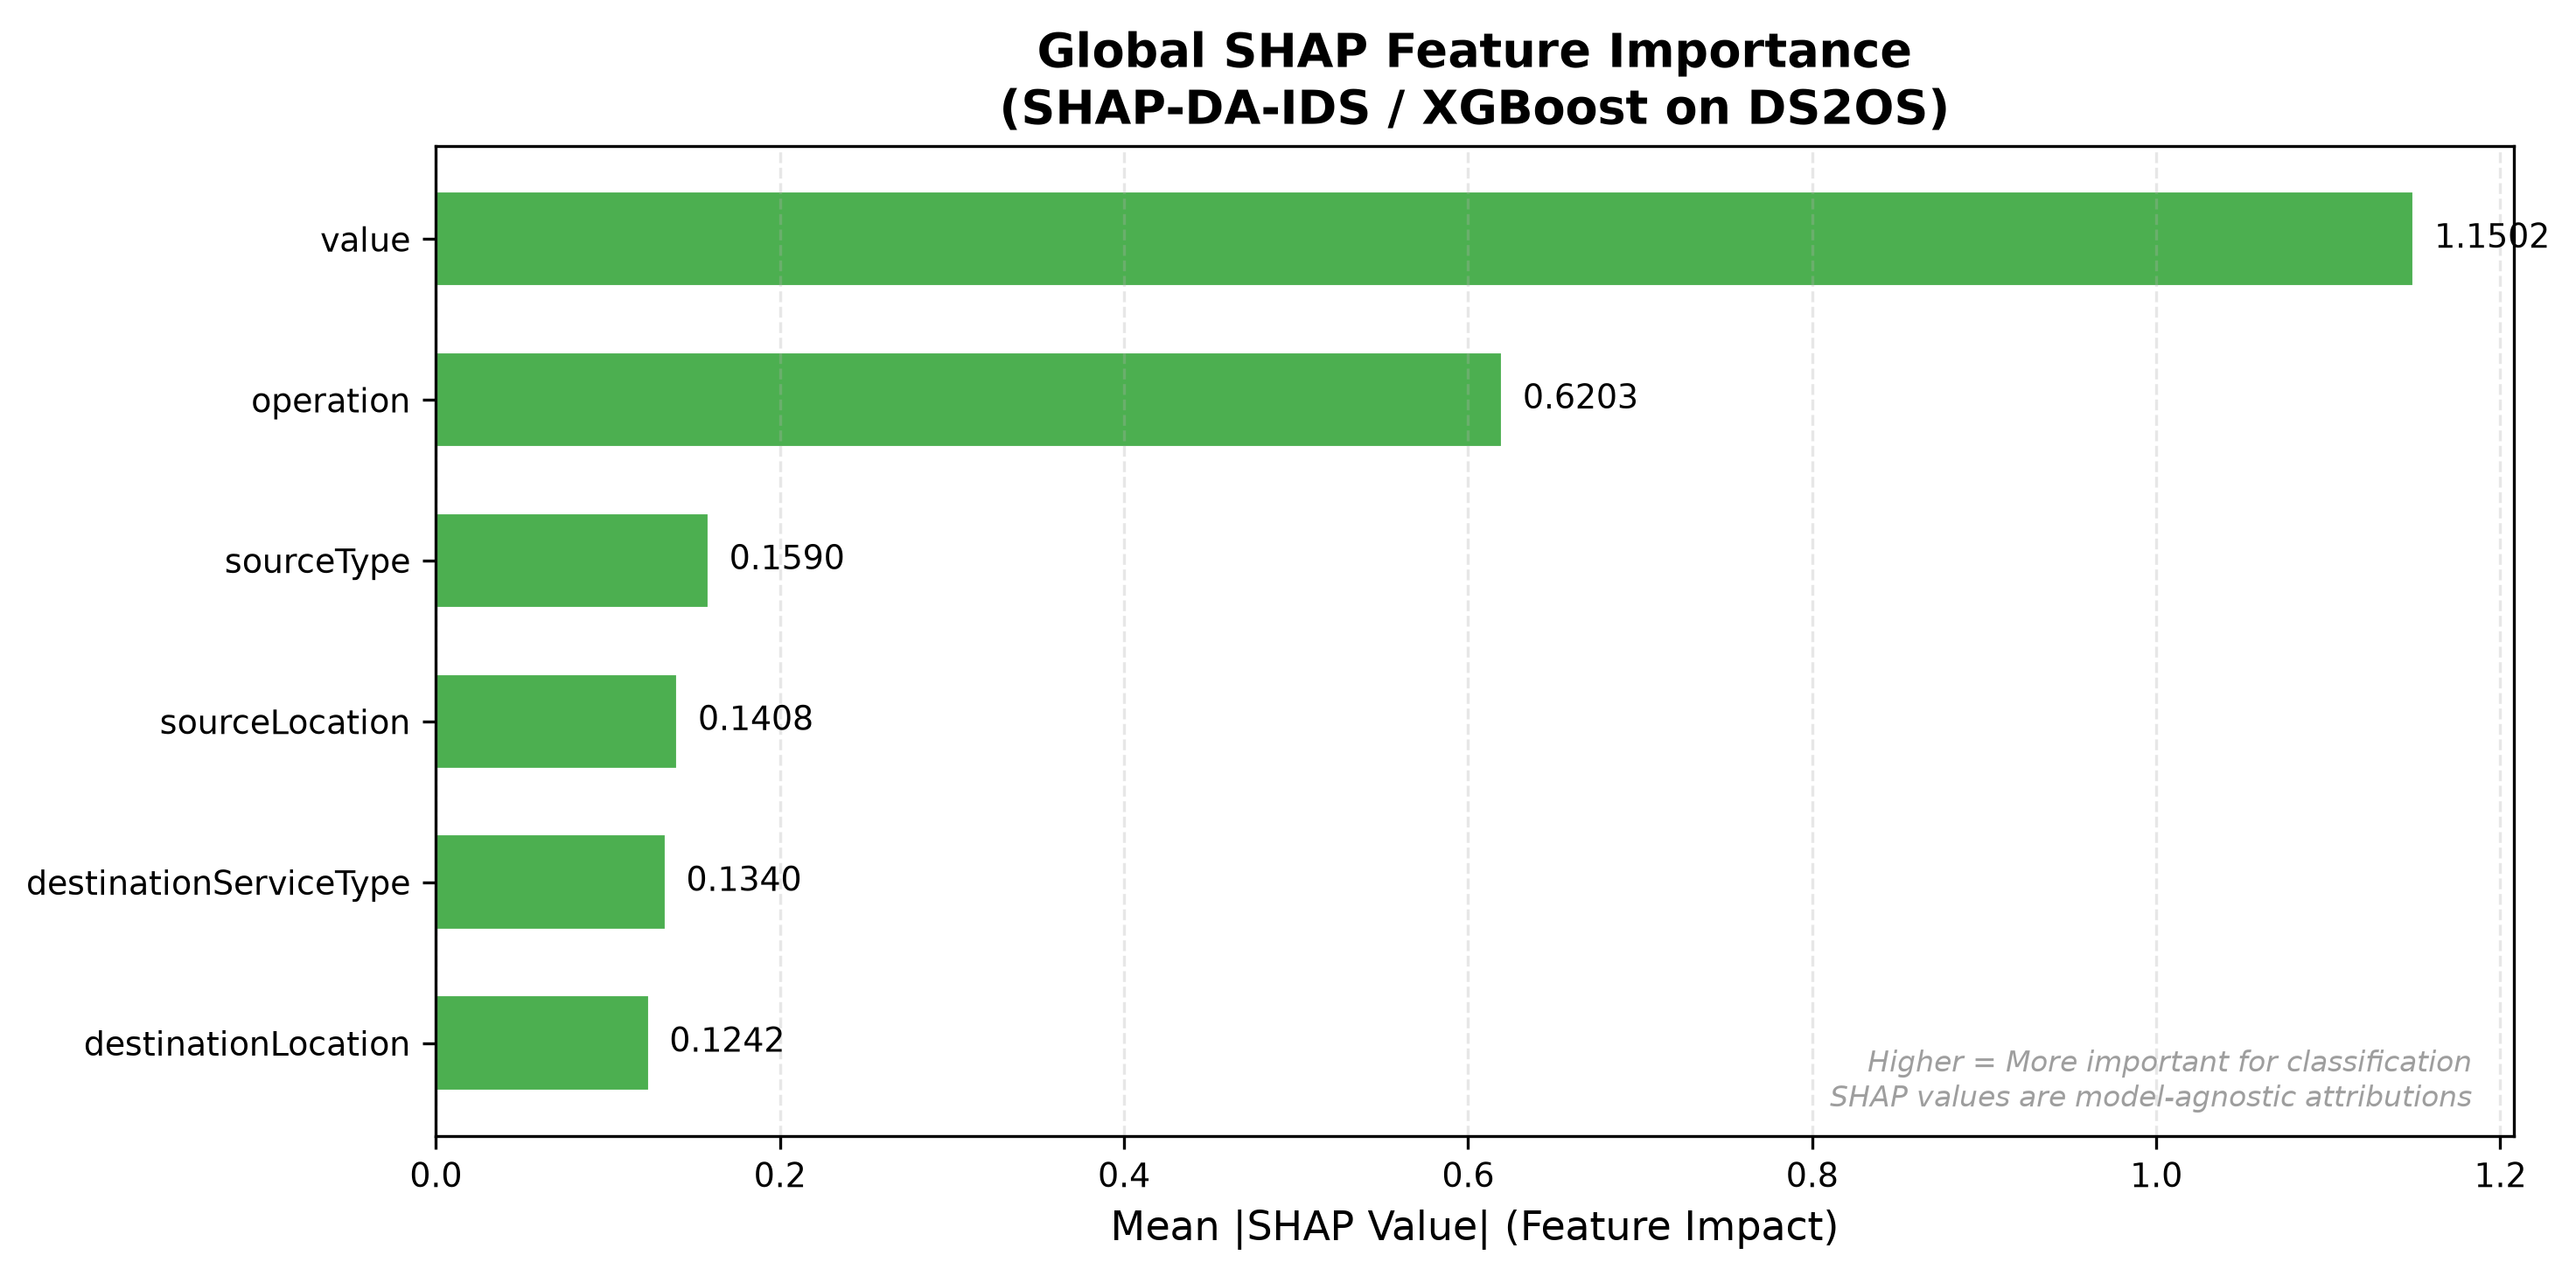
\includegraphics[width=\columnwidth]{images/6.png}
\caption{Global feature importance computed via TreeSHAP on test predictions, showing mean absolute Shapley attribution across retained network features.}
\label{fig:shap_importance}
\end{figure}

The Shapley values reveal two primary drivers of model decisions:
\begin{enumerate}
    \item \textbf{Payload Value (\texttt{value}, Mean $|\text{SHAP}| = 1.1502$):} The continuous sensor reading or telemetry payload is by far the most informative feature. Out-of-bound readings serve as strong indicators for data probing and setup tampering attacks.
    \item \textbf{Command Type (\texttt{operation}, Mean $|\text{SHAP}| = 0.6203$):} The specific function invoked (e.g., read, write, control) provides the second strongest signal. As shown in Table~\ref{tab:per_class_shap}, for DoS and Malicious Control, \texttt{operation} is the single most important feature, capturing rapid command loops and unauthorized actuation.
    \item \textbf{Device and Location Context:} Attributes such as \texttt{sourceType} and \texttt{sourceLocation} provide secondary discriminatory power, helping the model identify situations where an unprivileged sensor issues commands to a critical device.
\end{enumerate}

\begin{table}[!t]
\centering
\caption{Top Predictive Attribution Features Identified by SHAP per Attack Class}
\label{tab:per_class_shap}
\begin{tabular}{|l|l|}
\hline
\textbf{Class Label} & \textbf{Top Discriminative Features (Mean $|\text{SHAP}|$)} \\ \hline
Data Probing & \texttt{value}, \texttt{operation}, \texttt{sourceType} \\ \hline
DoS & \texttt{operation}, \texttt{value}, \texttt{sourceType} \\ \hline
Malicious Control & \texttt{operation}, \texttt{value}, \texttt{destinationLocation} \\ \hline
Malicious Operation & \texttt{operation}, \texttt{value}, \texttt{destinationServiceType} \\ \hline
Normal & \texttt{value}, \texttt{operation}, \texttt{sourceType} \\ \hline
Scan & \texttt{value}, \texttt{operation}, \texttt{sourceType} \\ \hline
Spying & \texttt{value}, \texttt{operation}, \texttt{sourceLocation} \\ \hline
Wrong Setup & \texttt{value}, \texttt{operation}, \texttt{sourceLocation} \\ \hline
\end{tabular}
\end{table}

\subsection{Computational Efficiency}
For edge IoT deployments, detection latency is as critical as accuracy. Table~\ref{tab:timing} compares the training time and test-set inference latency across models.

\begin{table}[!t]
\centering
\caption{Computational Resource Consumption on DS2OS Dataset}
\label{tab:timing}
\begin{tabular}{|l|c|c|}
\hline
\textbf{Model Architecture} & \textbf{Training Time (s)} & \textbf{Inference Latency (ms)} \\ \hline
Logistic Regression & \textbf{1.33} & \textbf{4.00} \\ \hline
Random Forest & 8.63 & 236.58 \\ \hline
XGBoost (Unbalanced) & 8.96 & 162.53 \\ \hline
XGBoost + Class Weights & 9.16 & 161.00 \\ \hline
XGBoost + Fixed (DIFT) & 9.15 & 158.64 \\ \hline
\textbf{SHAP-DA-IDS (Ours)} & 11.54 & 167.00 \\ \hline
\end{tabular}
\end{table}

SHAP-DA-IDS processes 71,591 test instances in 167.00\,ms, which corresponds to approximately 2.33\,$\mu$s per connection trace. This sub-millisecond per-packet latency indicates that the system can readily run on standard edge gateways and IoT hubs without requiring dedicated hardware accelerators.
